\section{Preliminaries}\label{sec2}
\subsection{Robot Model}
Consider a swarm $\mathcal{N}$ that contains $n$ robots labelled $i\in\left\{1,...,n\right\}$. The swarm is modeled as a directed sensing graph $\mathcal{G}=\left(\mathcal{V},\mathcal{E}\right)$, where vertex set $\mathcal{V} = \left\{1,..., n\right\}$ represents the robots, and edge set $\mathcal{E}\subseteq\mathcal{V}\times \mathcal{V}$ contains robot pairs $\left(i, j\right)\in\mathcal{E}$ in which robot $i$ can sense robot $j$. Denote $\mathcal{N}_i=\left\{j\in\mathcal{V}|\left(i,j\right)\in\mathcal{E}\right\}\subset\mathcal{V}$ as the set of $n_i$ neighbors of robot $i$ in $\mathcal{G}$.

\begin{figure}
    \centering
    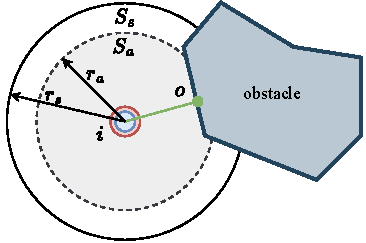
\includegraphics[width=0.45\textwidth]{paper2/images/model.pdf}
    \caption{Illustration of a robot with a local range sensor. Each robot is equipped with a local sensor with sensing area $S_s$ (solid while circle) being a circular disk within radius $r_s$. Additionally, alert area $S_a$ (dashed gray circle) is a circular disk within radius $r_a$, with $r_a\leq r_s$, which is the zone that robot will active the repulsive force to avoid collision. The set~$\mathcal{M}_i=\{o\}$ (green) is the nearest point from robot $i$ to obstacle.}
    \label{fig:1model}
\end{figure}

\begin{figure*}
    \centering
    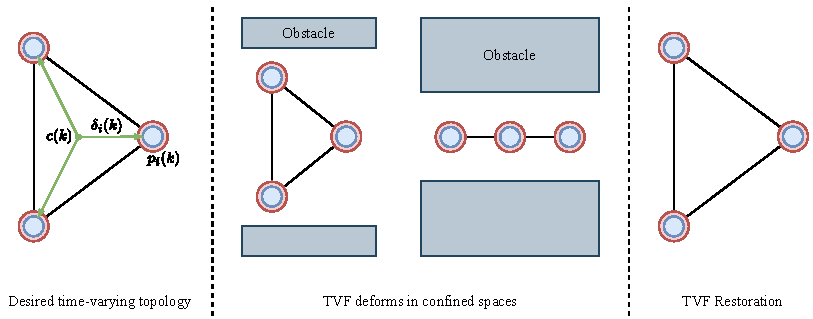
\includegraphics[width=0.9\textwidth]{paper2/images/problem.pdf}
    \caption{Schematic diagram of time-varying formation in the confined space}
    \label{fig:1problem}
\end{figure*}

In this work, robots in the swarm are identical, each with a body radius $r$. Each robot is equipped with an inertial measurement unit (IMU) to determine its position and orientation in a desired direction, a range sensor, and a wireless ad-hoc network module for peer-to-peer communication with other robots. The communication delay between any two robots is assumed to be negligible~\cite{AlonsoMora2018,9527169}. The range sensor has $360^\circ$ field of view providing a scanning area $S_s$ of radius $r_s$, as depicted in Figure~\ref{fig:1model}. The sensor data collected by robot $i$ at time $t(k)$ is represented as set $\mathcal{M}_i(k)$ of data points $o$ to obstacles, $\mathcal{M}_i(k) = \{o\}$. A safe area of radius $r_a$ is defined so that repulsive forces are activated when robot $i$ senses obstacles or its neighbors within range $r_a$.

The robot's dynamics is expressed in discrete time. Let $\tau$ be the time step, and $p_i(k), v_i(k), u_i(k) \in \mathbb{R}^3$  be the position, velocity, and control input of robot $i$ at time $t(k) = k\tau$, respectively. According to~\cite{Dong2015}, the robot's dynamics can be expressed by a discrete linear system as follows:
\begin{equation}
    x_i(k+1)=A_ix_i(k) + B_iu_i(k),
    \label{eqn:1model}
\end{equation}
where $A_i$ and $B_i$ are system matrices, $u_i$ is  acceleration input, and  $x_i=\left[p_i,v_i\right]^T\in\mathbb{R}^6$ is a state vector containing position and velocity. The velocities and accelerations are bounded so that $\left\Vert v_i(k)\right\Vert\leq v_\text{max}$ and $\left\Vert u_i(k)\right\Vert\leq u_\text{max}$.

\subsection{Problem formulation}

This paper addresses the time-varying formation (TVF) control for a swarm of robots in narrow spaces. Denote $\delta(k)$ as the desired formation configuration at time $k$. The TVF problem can be described via the following definitions~\cite{Dong2015,Dong2016}.

\begin{definition}\label{def_tvf}
Time-varying formation:  Let $\delta(k)=\left[\delta_1(k),...,\delta_n(k)\right]^T$ be a bounded time-varying vector that describes the desired formation configurations. The formation is said to achieve a TVF $\delta(k)$ if all robots in the formation satisfy:
\begin{equation}
    \lim_{k\to\infty}\sum_{i=1}^n\left( p_i(k)-\delta_i(k)-c(k)\right)=0
\end{equation}
where $c(k)$ is the formation center at time $k$.
\end{definition}

\begin{definition}\label{def_pro}
Safe formation: Given the TVF defined in Definition~\ref{def_tvf}, this TVF is said to be safe for any robot $i$, with $i\in\left\{1,...,n\right\}$ in the formation if the following conditions are satisfied:
\begin{enumerate}
    \item Formation configuration
\begin{equation}
    \lim_{k\to\infty}\sum_{j=1,j\neq i}^n{\left\Vert\left(p_i(k)-\delta_i\right) - \left(p_j(k)-\delta_{j}\right)\right\Vert}=0
    \label{eqn:form}
\end{equation}
%     \item Task completion
% \begin{equation}
%     \lim_{k\to T}\left\Vert\dfrac{1}{n}\sum_{i=1}^np_i-p_g\right\Vert=0
%     \label{eqn:goal}
% \end{equation}
% where $T$ is a finite time, $p_g$ is the target position.
    \item Safe distance between robots
\begin{equation}
    \left\Vert p_i(k)-p_j(k)\right\Vert > 2r
    \label{eqn:col}
\end{equation}
for all $j\neq i, j\in\left\{1,...,n\right\}$.
    \item Safe distance from obstacles
\begin{equation}
    \left\Vert p_i(k)-o\right\Vert > r
    \label{eqn:obs}
\end{equation}
for all $o\in\mathcal{M}_i(k)$. 
\end{enumerate}
\end{definition}

\begin{remark}
From Definition~\ref{def_tvf}, the robots reach their desired positions, hence achieving the desired configuration. In the decentralized approach, when~\eqref{eqn:form} is established, the system also ensures convergence to the desired configuration~\cite{Dong2015}.
% Simultaneously, the velocity tends to zero once the tasks are completed~\eqref{eqn:goal}. 
Conditions \eqref{eqn:col}~--~\eqref{eqn:obs} ensure collision avoidance both among robots within the formation and between any robot and surrounding obstacles.
\end{remark}

\subsection{Formation configurations}\label{sec:config}
Formation configurations refer to the shape that the robots form while cooperating and interacting with the environment. This work considers two following primary configurations:
\begin{enumerate}
    \item \textit{Desired configuration:} The desired configuration represents the arrangement that the robot swarm is expected to maintain to accomplish its task. Common desired configurations include shapes such as polygons and V-shapes.
    \item \textit{Straight line configuration:} This formation configuration is employed when the robots do not have enough space to maintain their original configuration. It is constructed by having a robot follow and keep desired distance from its leader.
\end{enumerate}